\begin{figure}
\centering
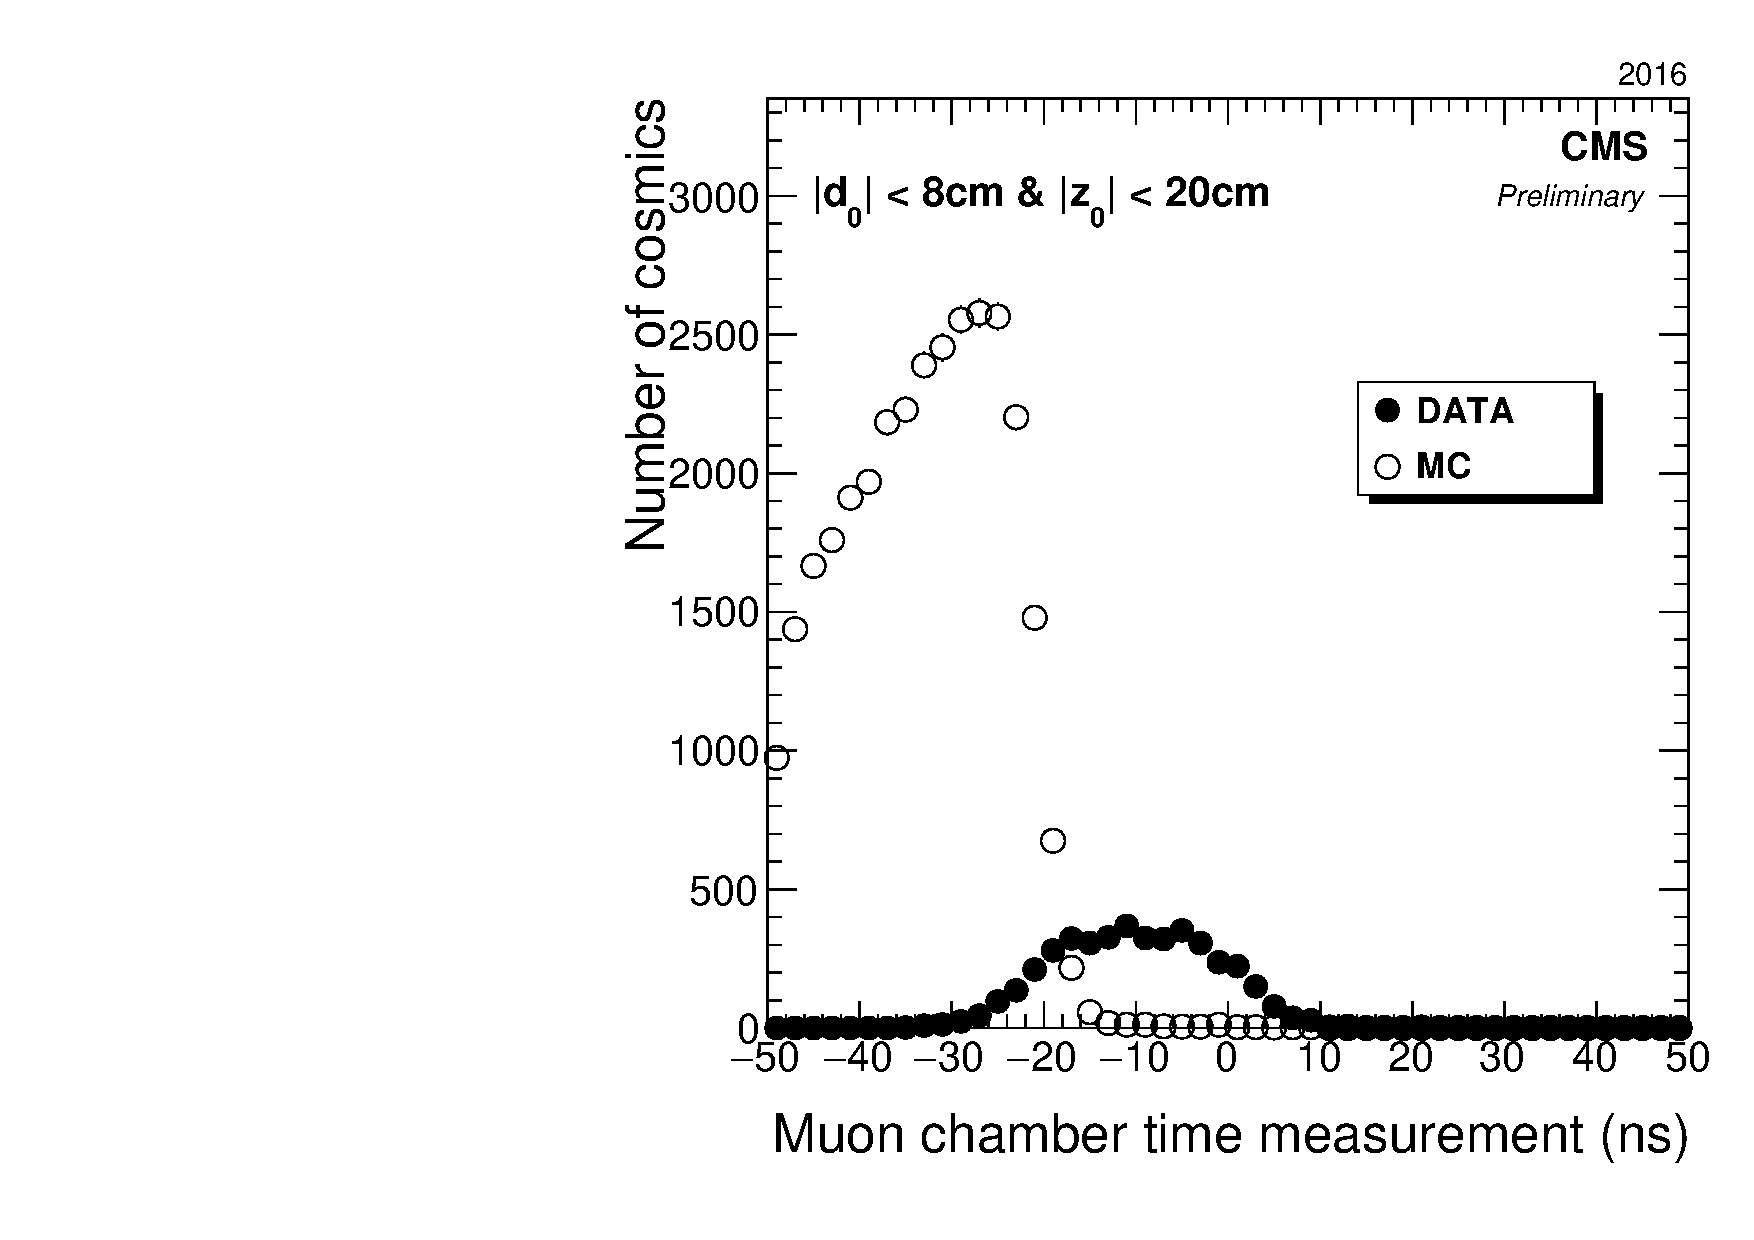
\includegraphics[width=0.32\textwidth]{figures/tracking_eff/2016/Muon2TimeAve.pdf}
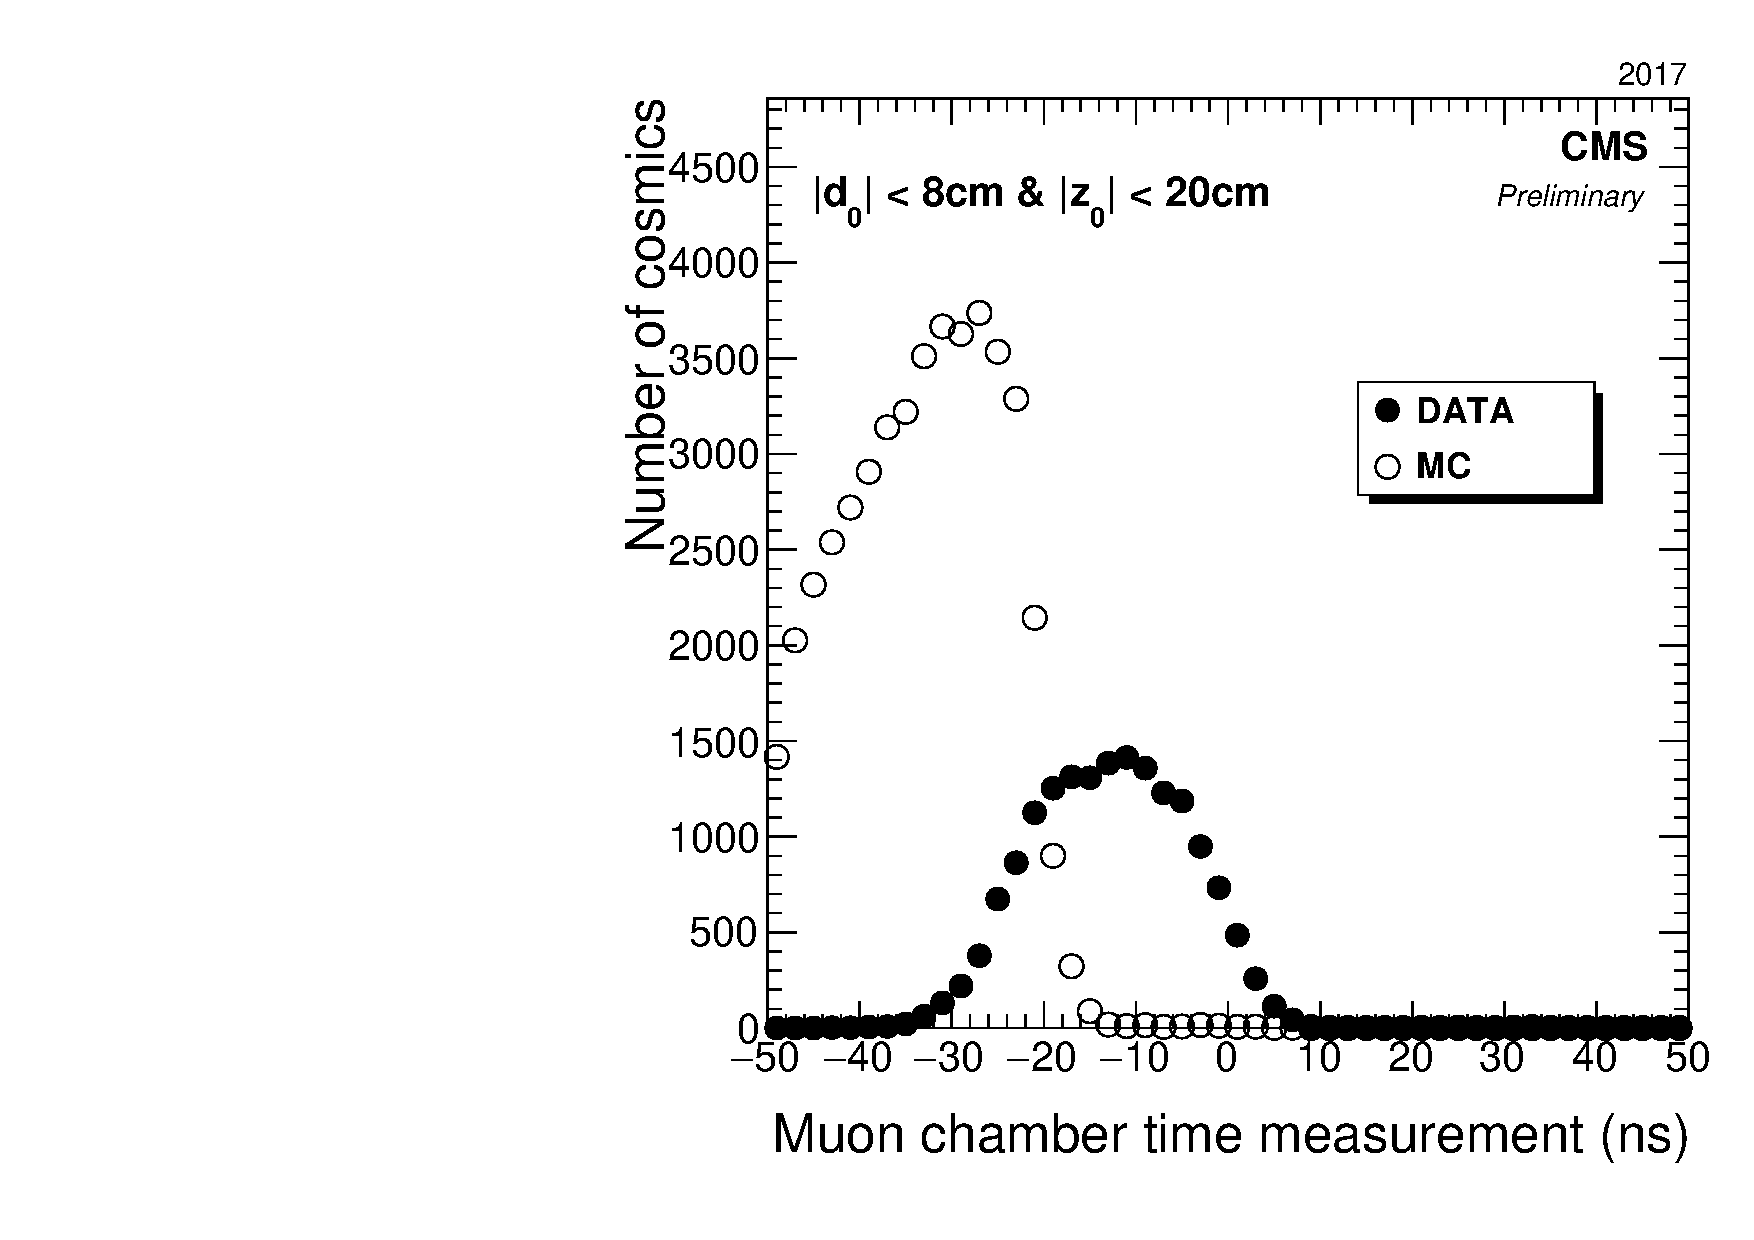
\includegraphics[width=0.32\textwidth]{figures/tracking_eff/2017/Muon2TimeAve.pdf}
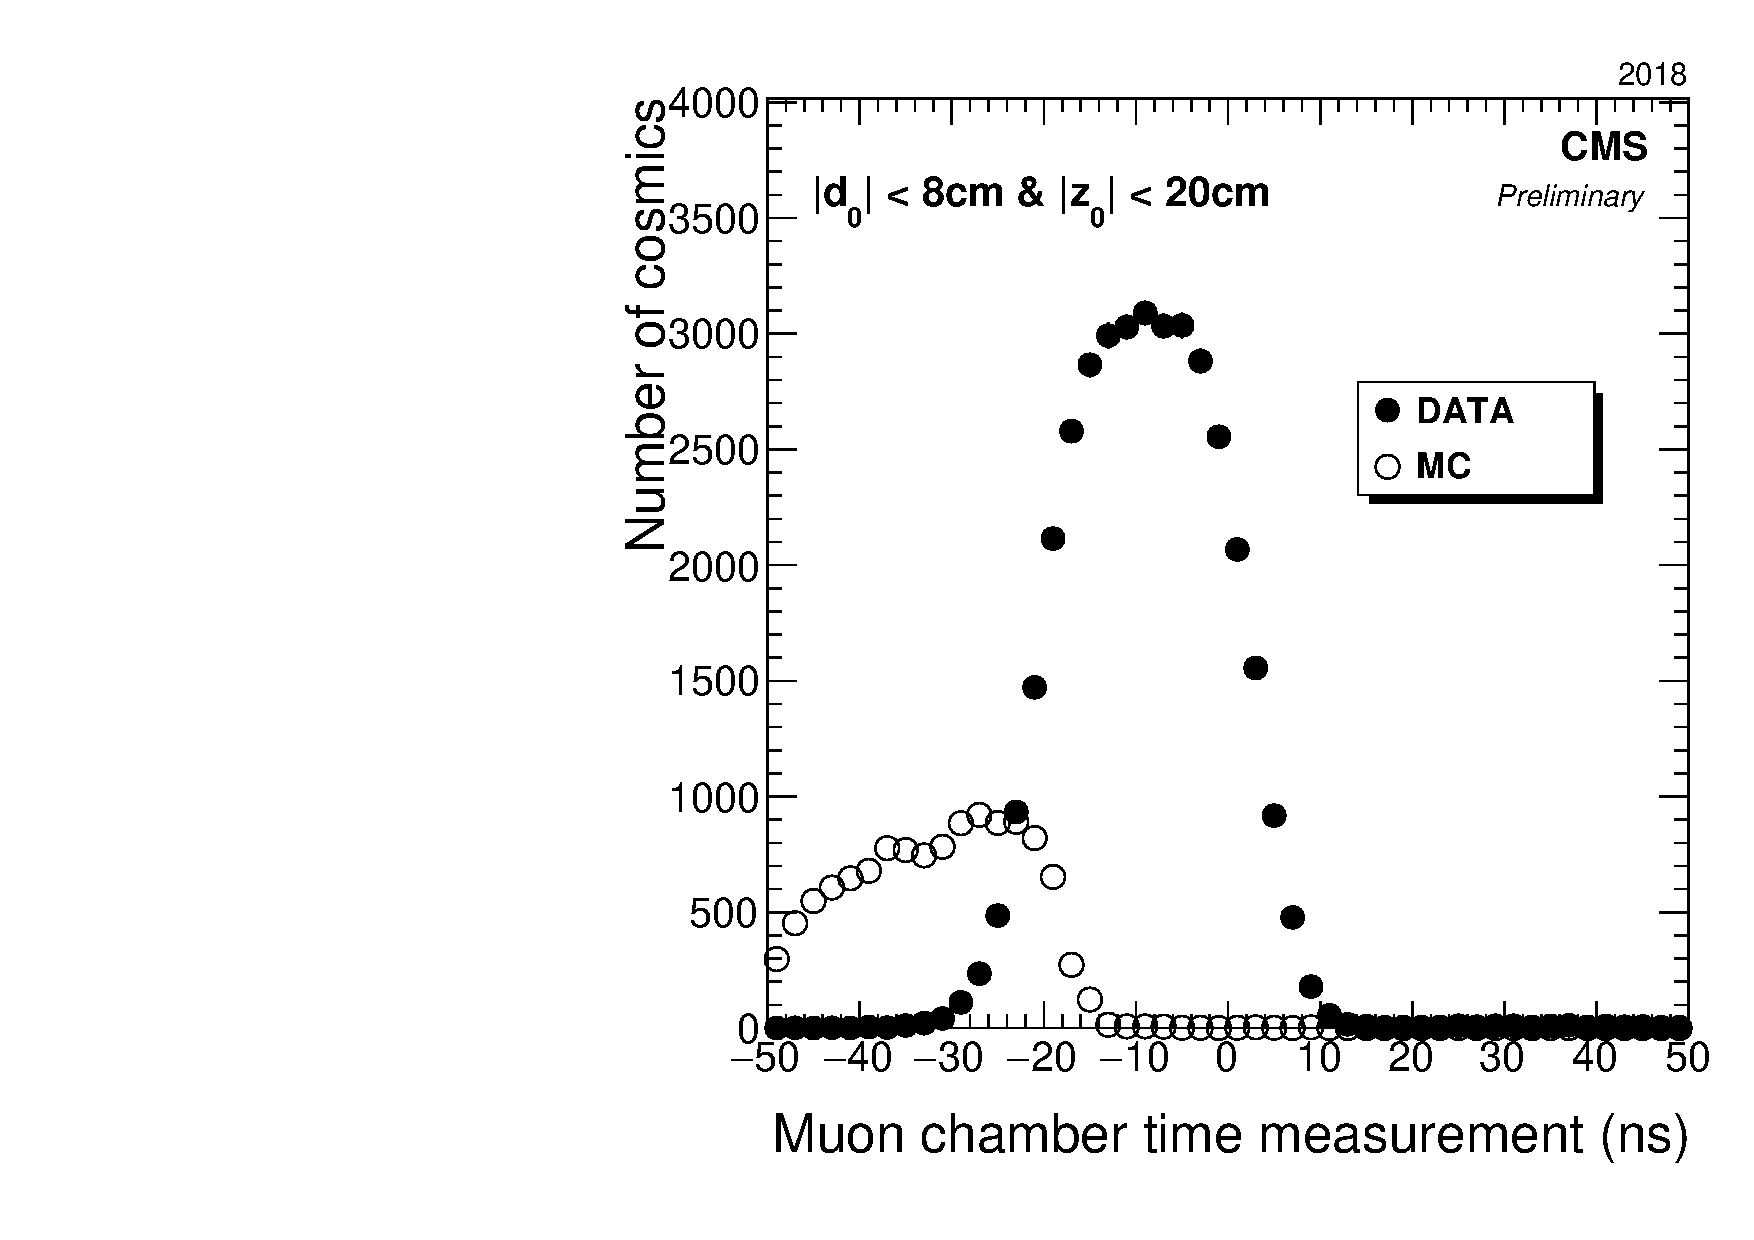
\includegraphics[width=0.32\textwidth]{figures/tracking_eff/2018/Muon2TimeAve.pdf}
\caption{Distribution of the arrival time of cosmic rays at their point of closest approach to the beamline as measured by the muon system in 2016 (left), 2017 (center), and 2018 (right) in data and simulation. Only cosmic ray muons with $\ad<\SI{8}{\cm}$ and $\az<\SI{20}{\cm}$ are considered.}
\label{arrival_time}
\end{figure}

\begin{figure}[hbtp]
\centering
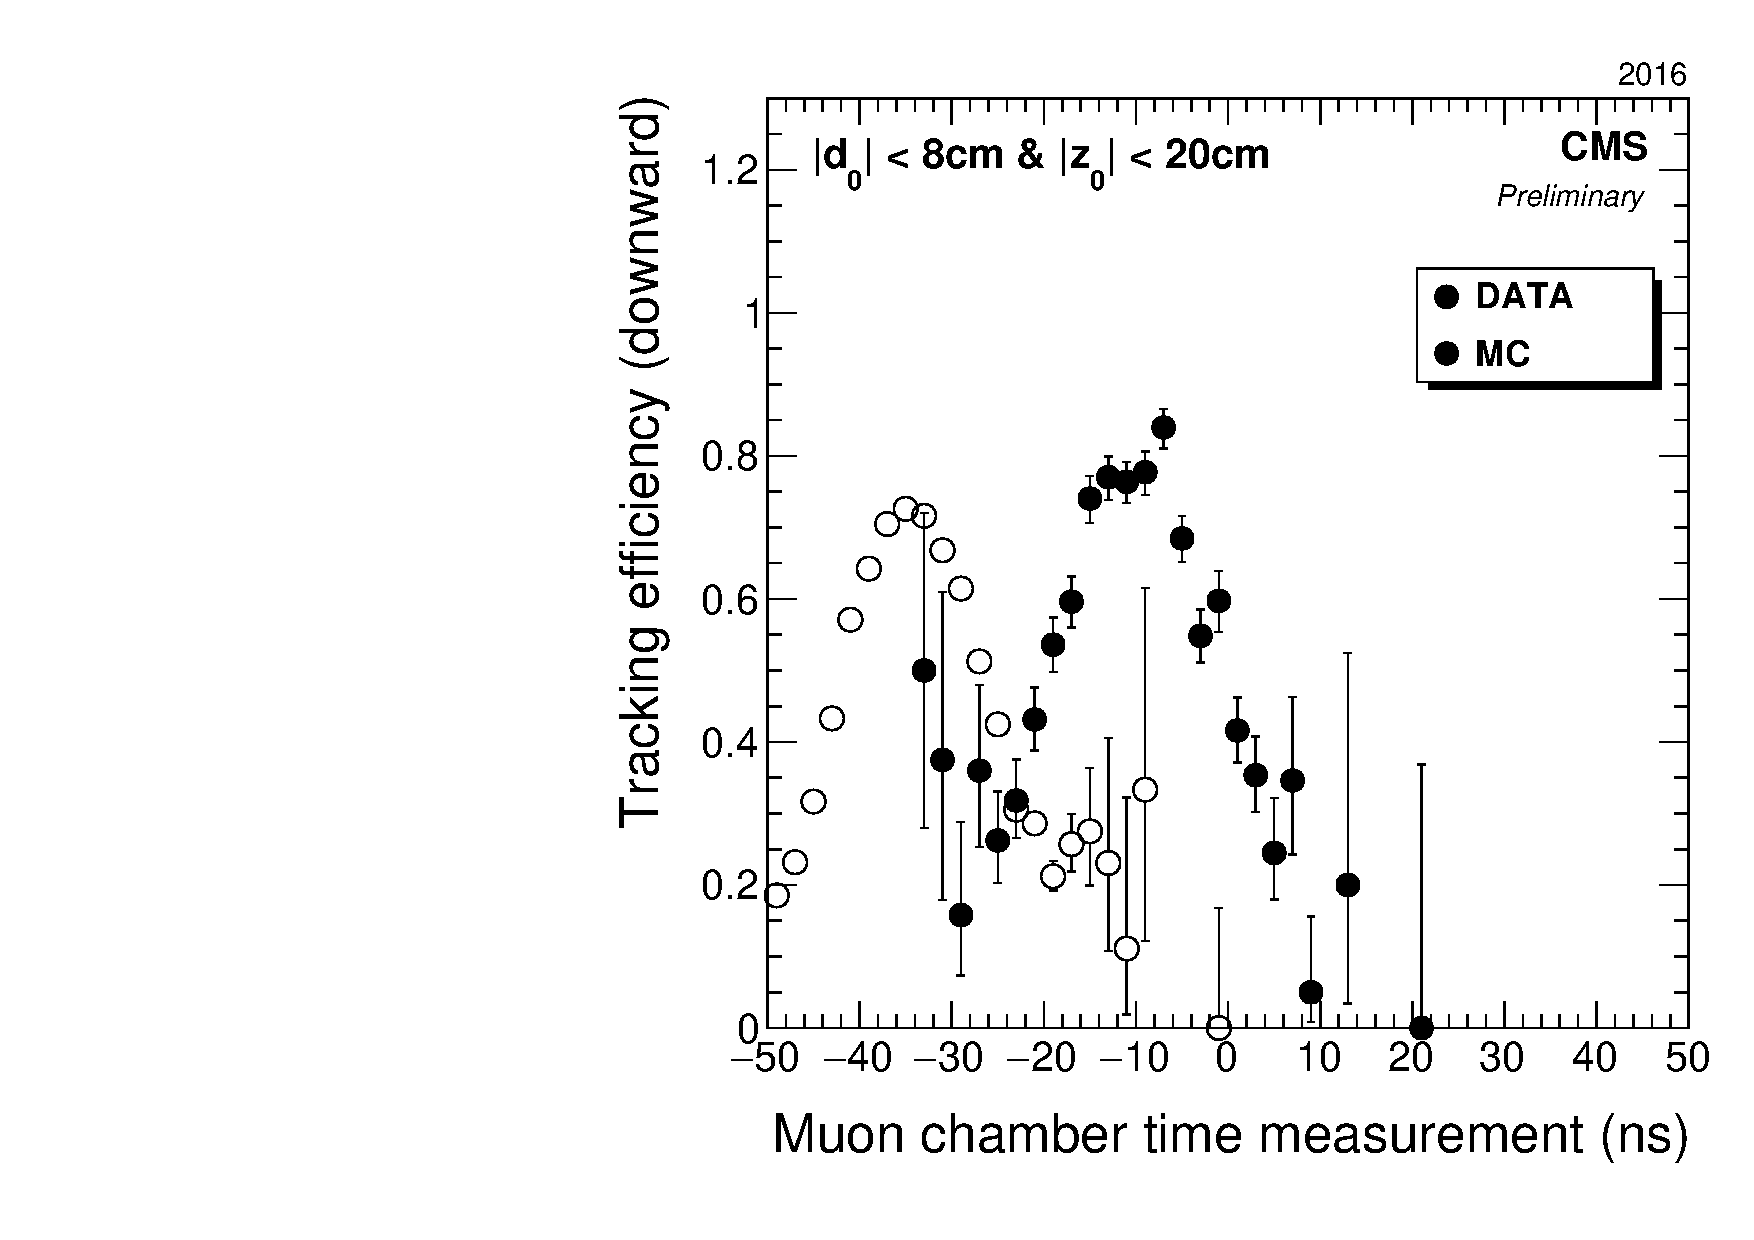
\includegraphics[width=0.32\textwidth]{figures/tracking_eff/2016/Eff0vsMuon2Time.pdf}
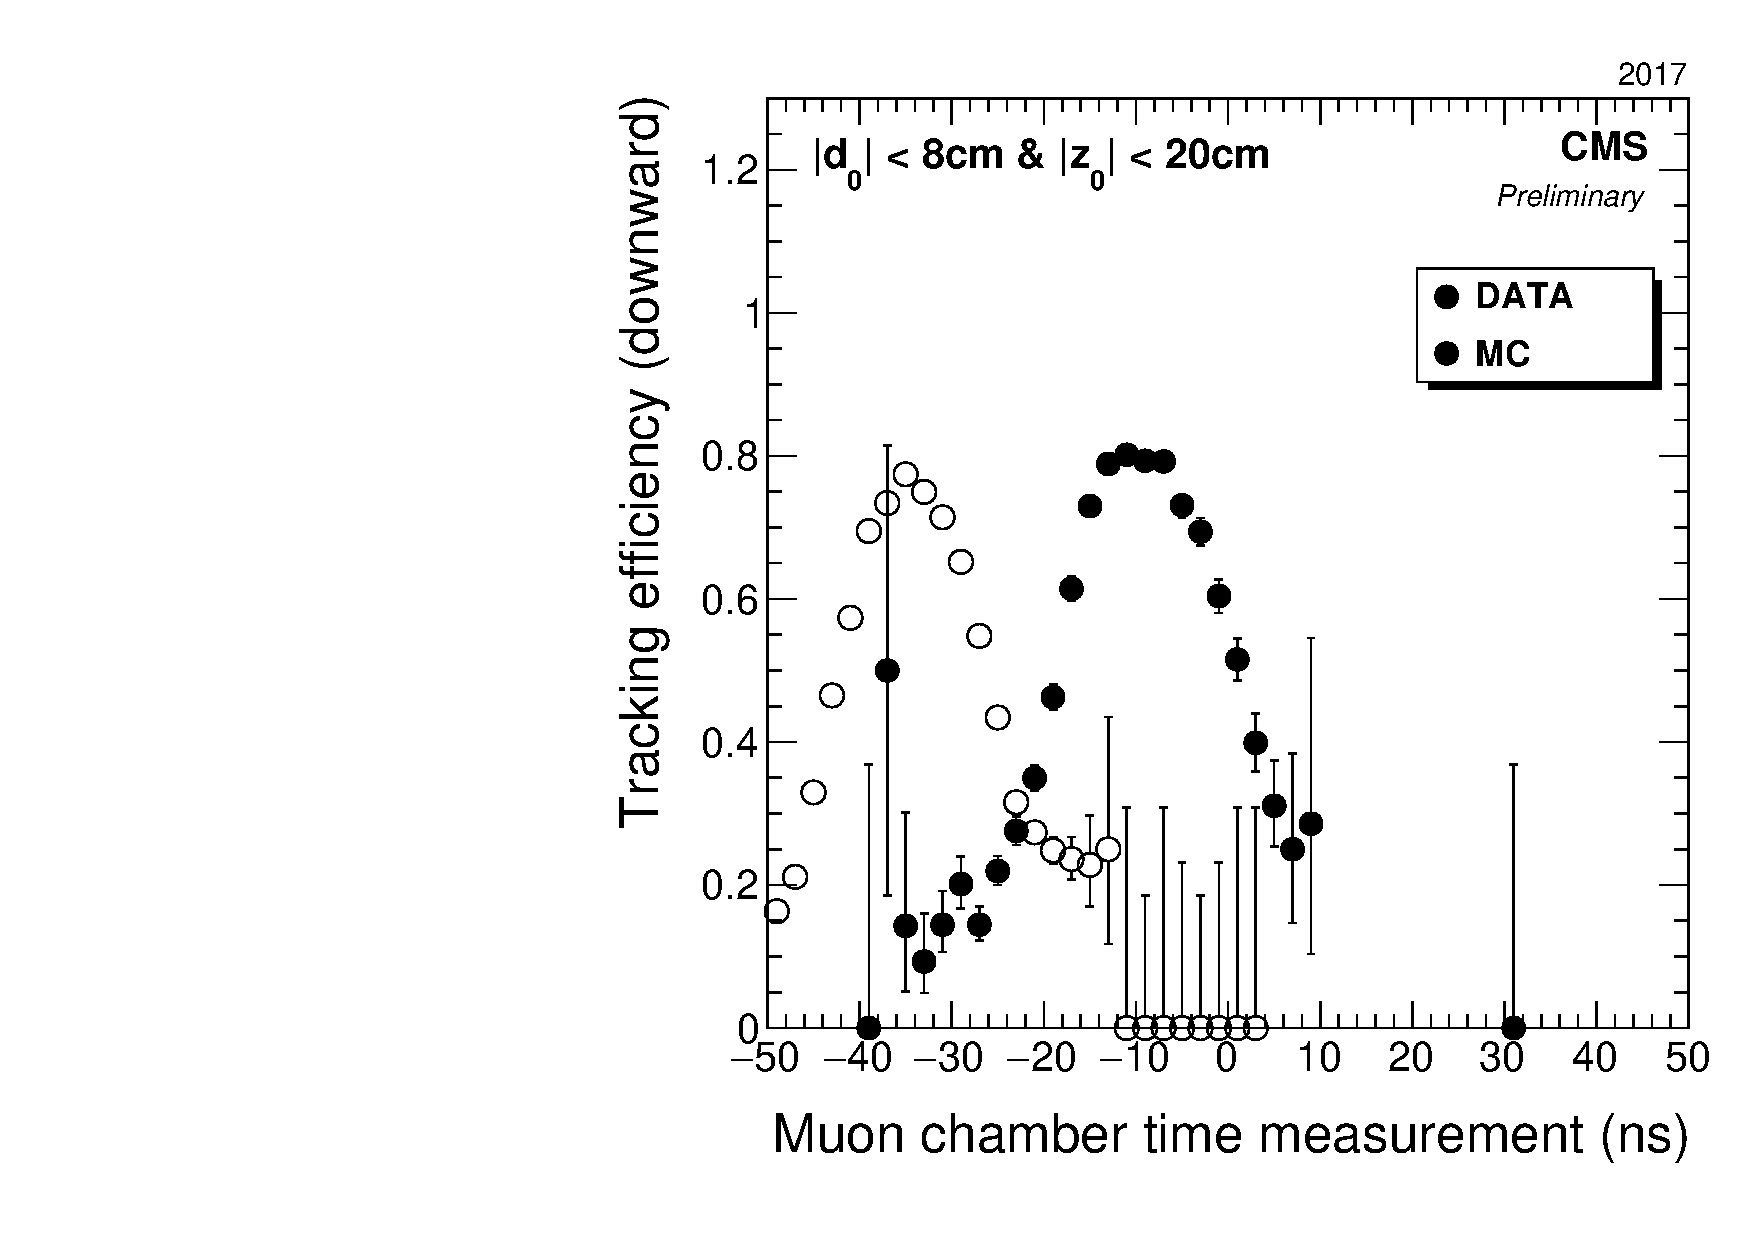
\includegraphics[width=0.32\textwidth]{figures/tracking_eff/2017/Eff0vsMuon2Time.pdf}
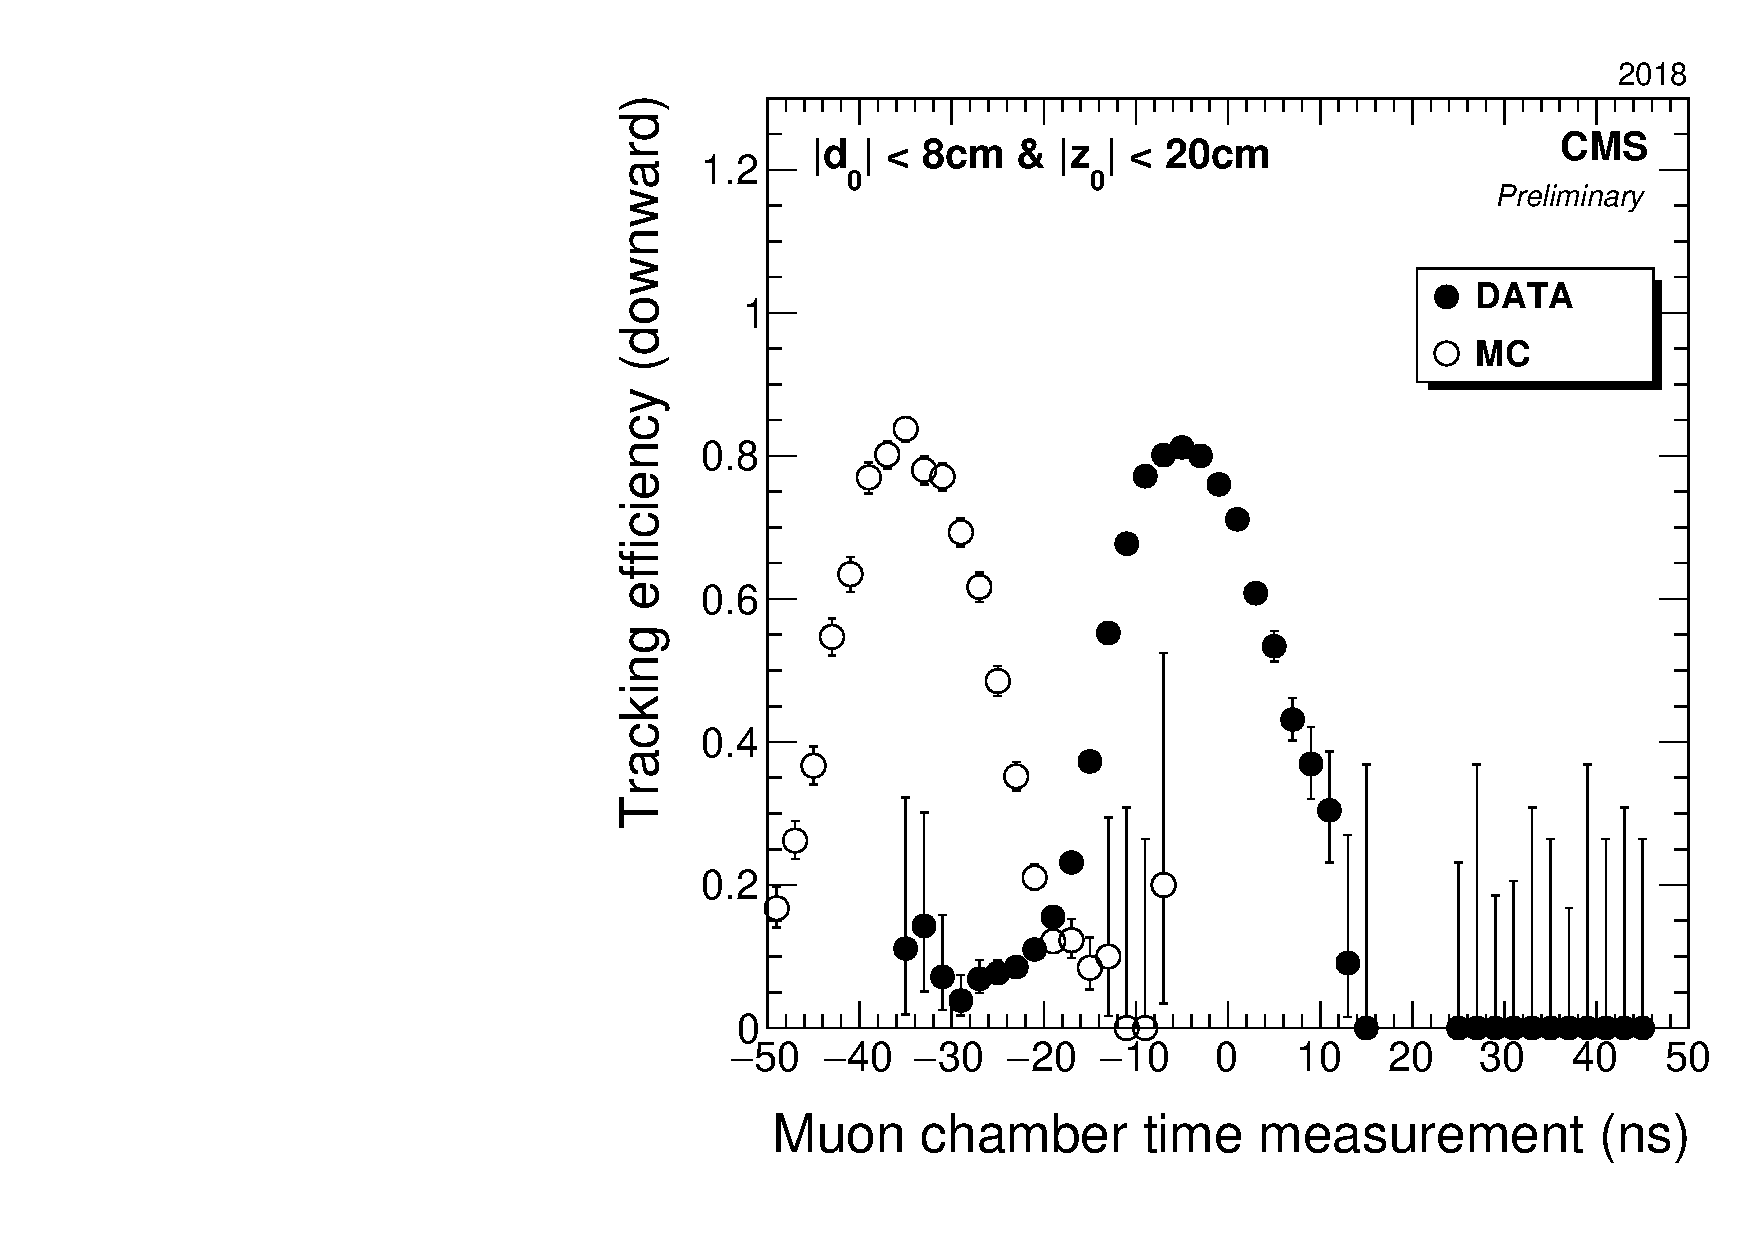
\includegraphics[width=0.32\textwidth]{figures/tracking_eff/2018/Eff0vsMuon2Time.pdf}
\caption{Measured downward tracking efficiency versus cosmic ray muon arrival time in 2016 (left), 2017 (center), and 2018 (right) in data and simulation. Only cosmic ray muons with $\ad<8$\cm and $\az<20$\cm are considered.}
\label{trk_eff_vs_arrival_time}
\end{figure}